\section{Entwurfsphase}
	
	Ziel:
	\begin{itemize}
		\item Aus \underline{gegebenen Anforderungen} an einem Softwareprodukt wird eine \newline \underline{softwaretechnische Lösung}, die \textbf{Softwarearchitektur}, entwickelt
	\end{itemize}
		
	\subsection{Softwarearchitektur}
			
		\begin{itemize}
			\item Gliederung eines Softwaresystems in \textbf{Komponenten} (Module, Klassen) und \textbf{Subsysteme} (Pakete, Bibliotheken)
			\item \textbf{Spezifikationen} der Komponenten und Subsystemen
			\begin{itemize}
				\item Aufstellung der \textbf{Benutztrelation}
			\end{itemize}
		\end{itemize}
		
	\subsection{Entwurfsmethoden}
			
		\begin{itemize}
			\item \textbf{Modularer Entwurf}
			\item \textbf{Objekt-orientierter-Entwurf}
			\begin{itemize}
				\item Erweiterung um Vererbung, Polymorphie und Datenmodellierung
			\end{itemize}
		\end{itemize}
	
	\subsection{Modul}
	
		\begin{itemize}
			\item Ist eine \textbf{Menge von Programmelementen} (Typen, Klassen, Konstanten, Variablen, Datenstrukturen, Prozeduren, Funktionen,..), die nach dem \textbf{Geheimnisprinzip} gemeinsam entworfen und geändert werden
		\end{itemize}
	
	\subsection{Anforderungen an ein Modul}
	
		\begin{itemize}
			\item Module sollen unabhängig voneinander bearbeitet und benutzt werden können
			\begin{itemize}
				\item \underline{Ohne Kenntnis} der späteren Nutzung entworfen, implementiert und getestet
			\end{itemize}
		\end{itemize}
		
	\newpage
	\subsection{Architekturstile}
			
		\begin{itemize}
			\item Schichtenarchitektur
			\item Klient/Dienstgeber (Client/Server)
			\item Partnernetze (Peer-To-Peer)
			\item Datenablage (Repository)
			\item Modell-Präsentation-Steuerung (Model-View-Controller)
			\item Fließband (Pipeline)
			\item Rahmenarchitektur (Framework)
			\item Dienstorientierte Architektur (Service oriented architecture)
		\end{itemize}
				
		\subsubsection{Schichtenarchitektur}
					
			\begin{itemize}
				\item Gliederung einer Softwarearchitektur mit \textbf{hierarchischen Schichten}
				\begin{itemize}
					\item Eine Schicht \underline{nutzt die darunter liegenden Schichten}  und diese \newline stellen ihre Dienste \underline{den darüber liegenden Schichten zur Verfügung}
				\end{itemize}
				\item Transparent:
			\end{itemize}						
			\begin{center}
				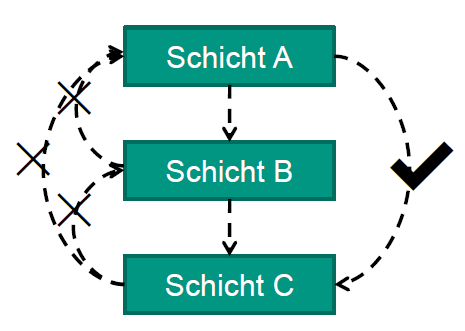
\includegraphics[width=0.5\textwidth]{../resources/images/transparenteSchichtenarchitektur.png}
			\end{center}					
			\newpage
			\begin{itemize}	
				\item Intransparent:	
			\end{itemize}				
			\begin{center}
				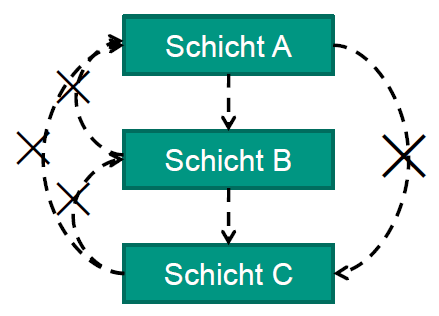
\includegraphics[width=0.5\textwidth]{../resources/images/intransparenteSchichtenarchitektur.png}
			\end{center}
			
			\begin{itemize}	
				\item 3-\textbf{stufige} Architektur
				\begin{itemize}
					\item 3-Schichten Architektur mit Schichten auf \underline{unterschiedlichen Rechnern}
				\end{itemize}
				\item 3-\textbf{Schichten} Architektur
				\begin{itemize}
					\item Benutzerschnittstelle, Anwendungskern und Datenbanksystem
				\end{itemize}
			\end{itemize}		
			Oft wird die Schichtenarchitektur mit dem Entwurfsmuster \textbf{Fassade} verwendet.
			\begin{itemize}
				\item Leitet an die eigentlichen Elemente in der Schicht weiter
			\end{itemize}				
			\begin{center}
				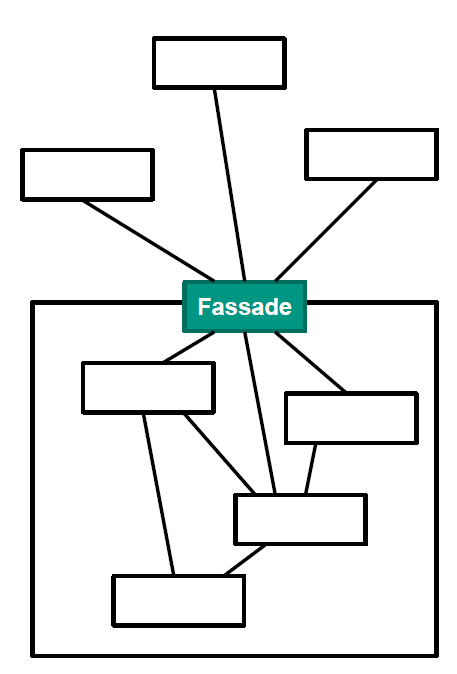
\includegraphics[width=0.3\textwidth]{../resources/images/fassadeSchichtenarchitektur.png}
			\end{center}
						
		\subsubsection{Klient/Dienstgeber}
						
			\begin{itemize}
				\item Ein- oder mehrere \textbf{Dienstgeber bieten Dienste für andere Subsysteme} (Klienten) an
				\begin{center}
					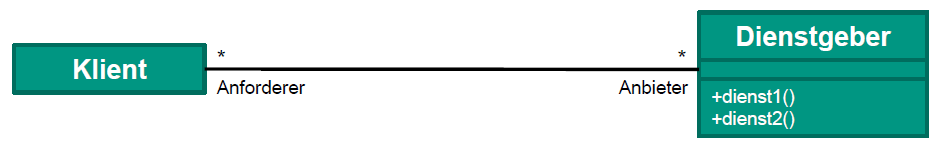
\includegraphics[width=0.9\textwidth]{../resources/images/klientDienstgeber.png}
				\end{center}
				\item Oft bei \textbf{Datenbankservern} verwendet
				\begin{itemize}
					\item \underline{Front-End:} Benutzeroberfläche für den Benutzer (Klient)
					\item \underline{Back-End}: Datenbankzugriff und Manipulation (Dienstgeber)
				\end{itemize}
				\item \textbf{Klientenfunktionen}
				\begin{itemize}
					\item Eingaben des Benutzer entgegennehmen und vor verarbeiten
				\end{itemize}
				\item \textbf{Dienstgeberfunktionen}
				\begin{itemize}
					\item Datenverwaltung, -integrität und -konsistenz
					\item Sicherheit
				\end{itemize}		
				\item Beispiel: TCP/IP, DNS (Netzwerkebene)		
			\end{itemize}	
			
		\subsubsection{Partnernetze}
					
			\begin{itemize}
				\item \textbf{Verallgemeinerung} von Klient/Dienstgeber
				\item Alle Subsysteme sind \textbf{gleichberechtigt}
				\begin{center}
					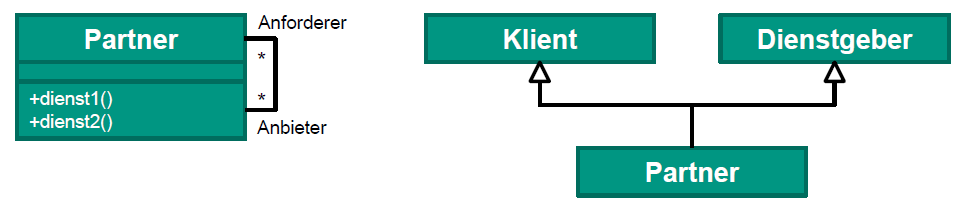
\includegraphics[width=0.9\textwidth]{../resources/images/partnernetze.png}
				\end{center}
			\end{itemize}
					
		\subsubsection{Datenablage}
					
			\begin{itemize}
				\item Subsysteme \textbf{verändern Daten} von einer zentralen Datenstruktur (Datenablage)
				\begin{itemize}
					\item Sind \textbf{lose gekoppelt} und interagieren nur über die Datenablage
				\end{itemize}
				\item Realisierung: \textbf{Lokaler- oder Fernzugriff}
				\begin{center}
					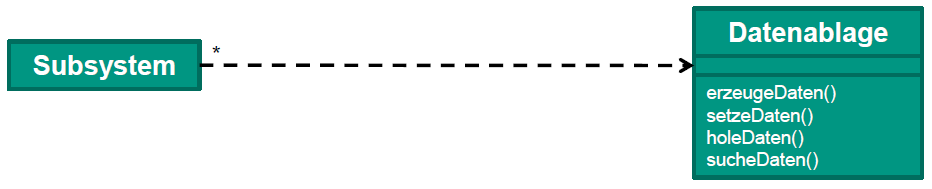
\includegraphics[width=0.9\textwidth]{../resources/images/datenablage.png}
				\end{center}
				\item Beispiele: Subversion, GIT
			\end{itemize}
			
		\subsubsection{Modell-Präsentation-Steuerung}
					
			\begin{center}
				\begin{tabular}{c|c}
					\textbf{Problem}                      & \textbf{Lösung} \\
					\hline
					System mit \underline{hoher Kopplung} & MVC mit \textbf{Trennung} von Daten und Darstellung
				\end{tabular}
			\end{center}
						
			\begin{itemize}
				\item \textbf{Modell:}
				\begin{itemize}
					\item Verantwortlich für \underline{anwendungsspezifische Daten}
				\end{itemize}
				\item \textbf{Präsentation:}
				\begin{itemize}
					\item Verantwortlich für die \underline{Darstellung} der Objekte der Anwendung
				\end{itemize}
				\item \textbf{Steuerung:}
				\begin{itemize}
					\item Verantwortlich für \underline{Benutzerinteraktion}
					\item \underline{Aktualisiert} Modell
					\item Weiterleitung der \underline{Änderung von Modelldaten} an Präsentation
				\end{itemize}
				$\Rightarrow$ Entwurfsmuster: \textbf{Beobachter}!
			\end{itemize}	
			\begin{center}
				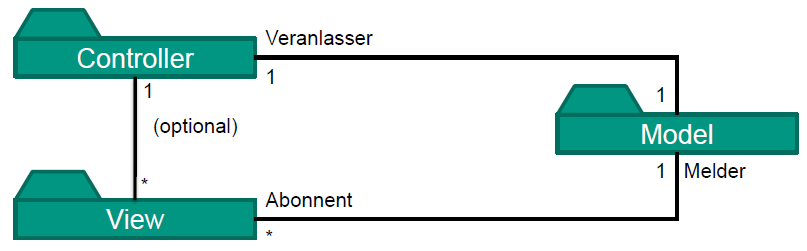
\includegraphics[width=0.9\textwidth]{../resources/images/mvc.png}
			\end{center}
			
		\subsubsection{Fließband}
					
			\begin{itemize}
				\item Jede/r Stufe/Filter ist ein \textbf{eigenständiger- und ablaufender Prozess/Faden}
				\item Jede Stufe \textbf{verarbeitet vorherige Daten} und sendet sie an die nächste Stufe
			\end{itemize}
				
			\begin{center}
				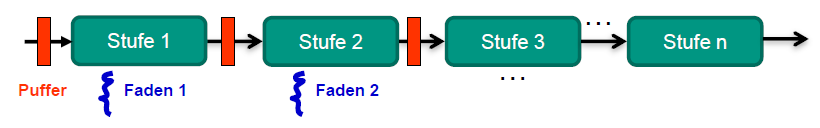
\includegraphics[width=0.8\textwidth]{../resources/images/fliessband.png}
				Bei Parallelrechnern echt parallel ausführbar!
			\end{center}
				
			\begin{itemize}
				\item Beispiel: Unix-Shell
				\item \textbf{Anwendung:}
				\begin{itemize}
					\item Datenströme (Videobearbeitung, Übersetzer, Stapelverarbeitung)
					$\Rightarrow$ Für \textbf{gute Leistung}: Einzelne Stufen etwa \underline{gleich schnell} ausführbar auf Parallelrechnern
				\end{itemize}
			\end{itemize}
			
		\subsubsection{Rahmenarchitektur}
					
			\begin{itemize}
				\item Bietet \textbf{fast vollständiges Programm}, dass durch \textbf{Lücken/Erweiterungen} erweitert werden kann
				\item \textbf{Klassenabstrahierung} und \textbf{Methodenüberschreibung} vorgesehen
				\begin{itemize}
					\item Rahmenprogramm führt Erweiterungen (\textbf{Plug-Ins}) richtig aus
				\end{itemize}
			\end{itemize}
						
			\underline{Herkömmlich:}
			\begin{itemize}
				\item Hersteller liefert Bibliotheken
				\item Benutzer schreibt Hauptprogrammlogik
			\end{itemize}				
			\begin{center}
				
\includegraphics[width=0.8\textwidth]{../resources/images/rahmenarchitekturHerkoemmlich.png}
			\end{center}
				
			\underline{Mit Rahmenarchitektur:}
			\begin{itemize}
				\item \textbf{Hollywood-Prinzip}: Don't call us, we call you!
				\item Hauptprogramm vorhanden, Erweiterungen vom Benutzer werden aufgerufen
			\end{itemize}				
			\begin{center}
				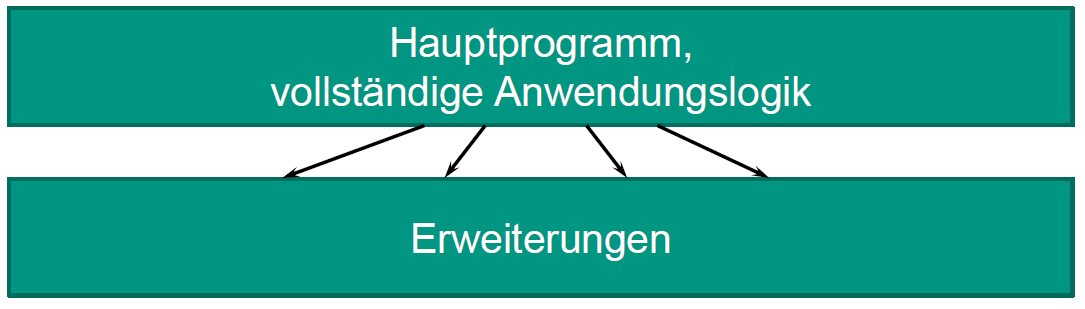
\includegraphics[width=0.8\textwidth]{../resources/images/rahmenarchitektur.png}
			\end{center}
				
			\newpage
			\underline{Beispiel:}				
			\begin{center}
				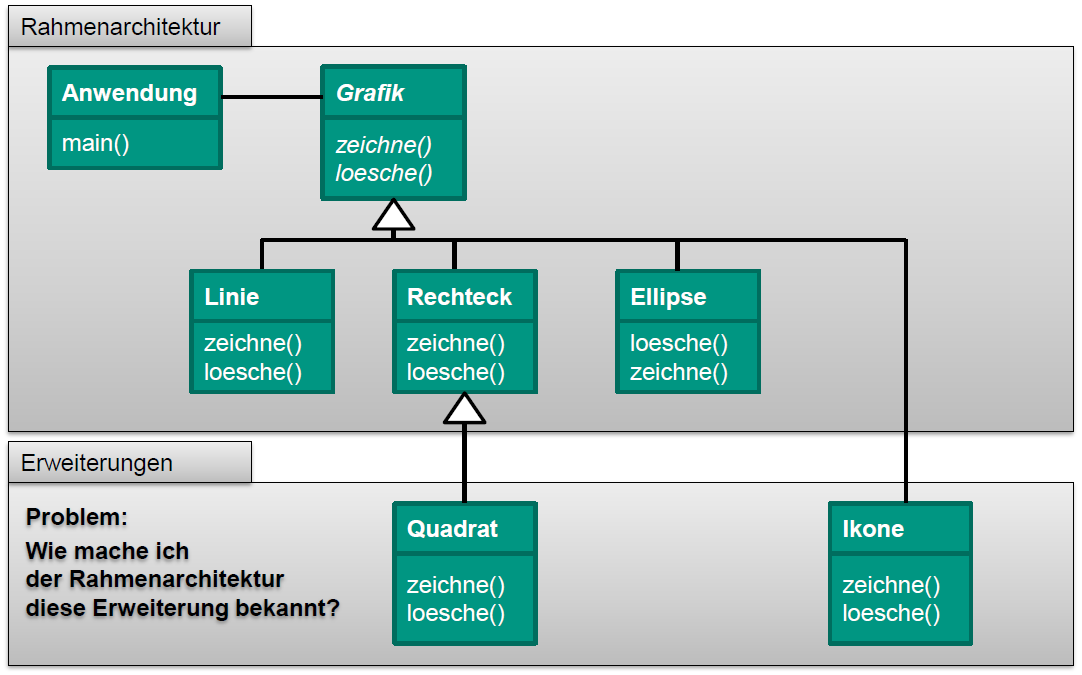
\includegraphics[width=0.9\textwidth]{../resources/images/rahmenarchitekturBeispiel.png}
			\end{center}
		
			\begin{itemize}
				\item \textbf{Anwendung:}
				\begin{itemize}
					\item \underline{Grundversion} der Anwendung schon funktionsfähig
					\item Erweiterung \underline{konsistent}
					\item \textbf{Entwurfsmuster:} Strategie, Fabrikmethode, Abstrakte Fabrik und Schablonenmethode
				\end{itemize}
			\end{itemize}
			
		\subsubsection{Dienstorientierte Architekturen}
				
			\begin{itemize}
				\item Anwendungen bestehen aus \textbf{unabhängigen Diensten}
				\begin{itemize}
					\item Abstraktes Konzept
				\end{itemize}
				\item Dienste als \textbf{zentrale Elemente} eines Unternehmens
				\begin{itemize}
					\item Bereitstellen gekapselter Funktionalität an andere Dienste/Anwendungen
					\begin{itemize}
						\item \textbf{Gemeinsame Schnittstelle} für standardisierte(r) Austausch/Kommunikation
					\end{itemize}
				\end{itemize}
				\item \underline{Merkmale/Ziele:}
				\begin{itemize}
					\item \textbf{Lose Kopplung}
					\begin{itemize}
						\item \underline{Einfaches Ersetzen} eines Dienstes zur Laufzeit
						\item \underline{Dynamisches Binden} durch Dienstverzeichnis
					\end{itemize}
					\item \textbf{Unterstützung von Geschäftsprozessen}
					\begin{itemize}
						\item Dienste kapseln geschäftsrelevante Funktionalität
					\end{itemize}
					\item \textbf{Verwendung von offenen Standards!}
					\begin{itemize}
						\item \underline{Programmiersprachen}- und \underline{plattformunabhängige} Bereitstellung von Diensten
					\end{itemize}
				\end{itemize}
			\end{itemize}		
			\begin{center}
				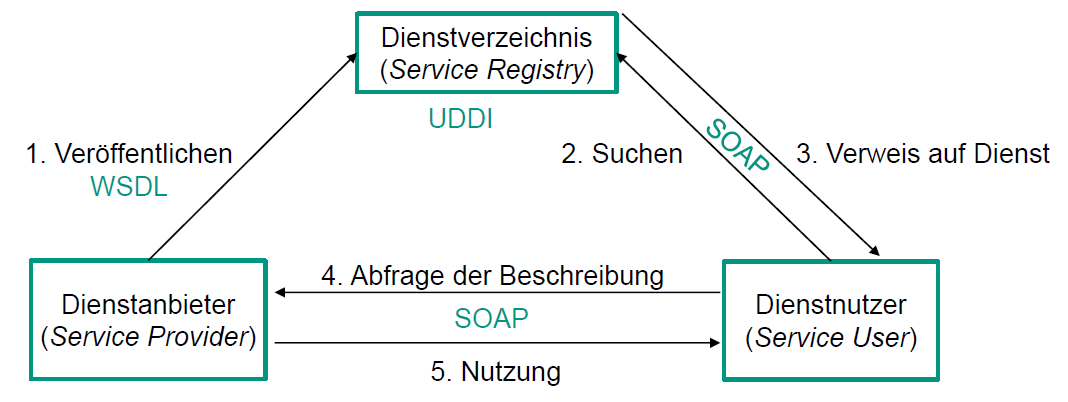
\includegraphics[width=0.9\textwidth]{../resources/images/dienstorientierteArchitektur.png}				
				$\Rightarrow$ \textbf{Dienstmodell} als Kern der Dienstorientierten Architektur
			\end{center}
	
	\subsection{Entwurfsmuster}
						
		\resizebox{\textwidth}{!}{
		\begin{tikzpicture}[mindmap, grow cyclic, text centered, every node/.style=concept, concept color=blue!60, level 1/.append style={text width=2.5cm, level distance=5.5cm,sibling angle=72}, level 2/.append style={text width=1.75cm, level distance=3.25cm,sibling angle=40}] 
						
		\node{Entwurfsmuster}
			child {node {Entkopplungs\\muster}
			child {node {Adapter}}
			child {node {Beobachter}}
			child {node {Brücke}}
			child {node {Iterator}}
			child {node {Stell\\vertreter}}
			child {node {Vermittler}}
			}
			child { node {Steuerungs\\muster}
			child {node {Befehl}}
			child {node {Master/\\Worker}}
			}
			child { node {Zustands\\handhabungs\\muster}
			child {node {Einzel\\stück}}
			child {node {Prototyp}}
			child {node {Memento}}
			child {node {Fliegen\\gewicht}}
			child {node {Zustand}}
			}
			child { node {Varianten\\muster}
			child {node {Abstrakte\\Fabrik}}
			child {node {Dekorierer}}
			child {node {Strategie}}
			child {node {Kompo\\situm}}
			child {node {Besucher}}
			child {node {Fabrik\\methode}}
			child {node {Schablonen\\methode}}
			}
			child { node {Bequemlich\\keitsmuster}
			child {node {Null-Objekt}}
			child {node {Fassade}}
			child {node {Bequem\\lichkeits\\methode}}
			child {node {Bequem\\lichkeits\\klasse}}
			};
		\end{tikzpicture}}
			
		\newpage
		\begin{itemize}
			\item \textbf{Entkopplungsmuster:}
			\begin{itemize}
				\item Teilt System in \textbf{unabhängige Einzelsysteme}
				\begin{itemize}
					\item \underline{Vorteil}: Durch lokale Änderungen \textbf{verbesser}-, \textbf{anpass}- und \textbf{erweiterbar} \underline{ohne} ganzes System zu modifizieren
				\end{itemize}
			\end{itemize}
			\item \textbf{Variantenmuster:}
			\begin{itemize}
				\item \textbf{Herausziehen von Gemeinsamkeiten} und platzieren an \underline{einer} Stelle
				\begin{itemize}
					\item \underline{Vorteil}: \textbf{Keine Codewiederholung}
				\end{itemize}
			\end{itemize}
			\item \textbf{Zustandshandhabungsmuster:}
			\begin{itemize}
				\item \textbf{Bearbeitung des Zustands} von Objekten unabhängig vom Zweck
			\end{itemize}
			\item \textbf{Steuerungsmuster:}
			\begin{itemize}
				\item \textbf{Kontrollflusssteuerung} (Aufruf der richtigen Methode zur richtigen Zeit)
			\end{itemize}
			\item \textbf{Bequemlichkeitsmuster:}
			\begin{itemize}
				\item \underline{Sparen} von \textbf{Schreib- und Denkarbeit}
			\end{itemize}
		\end{itemize}
		
		\newpage
		\subsubsection{Entkopplungsmuster}
						
			\begin{itemize}
				\item \textbf{Adapter} (Wrapper)
				\begin{itemize}
					\item \textbf{Passt die Schnittstelle einer Klasse an} eine andere, \textbf{vom Klienten erwartete Schnittstelle} an
				\end{itemize}
				\begin{center}
					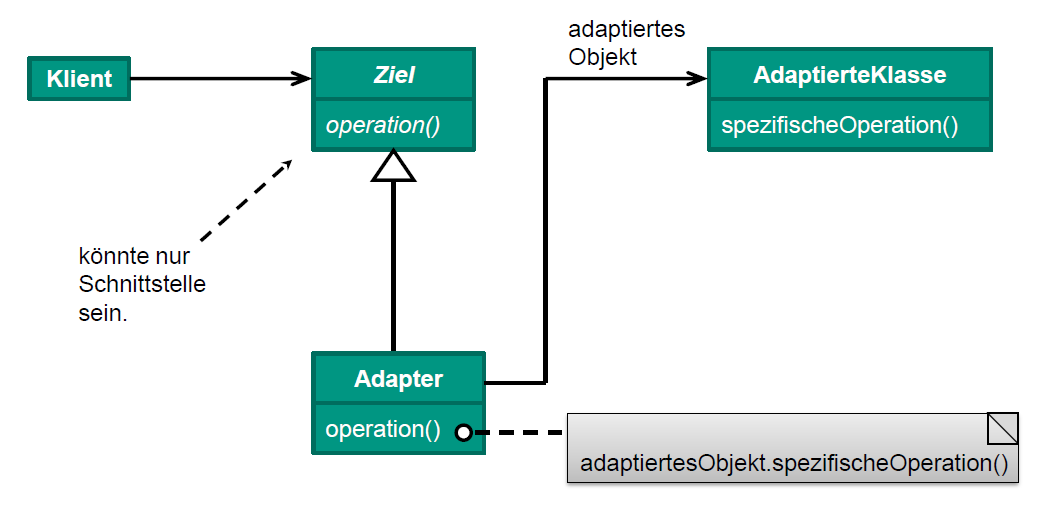
\includegraphics[width=0.9\textwidth]{../resources/images/adapter.png}
				\end{center}
				\item \textbf{Beobachter} (Observer)
				\begin{itemize}
					\item \textbf{1:n Abhängigkeit} zwischen Objekten, so dass die \textbf{Änderung eines Zustandes} eines Objektes dazu führt, dass alle abhängigen Objekte \textbf{benachrichtigt und aktualisiert} werden
				\end{itemize}
				\begin{center}
					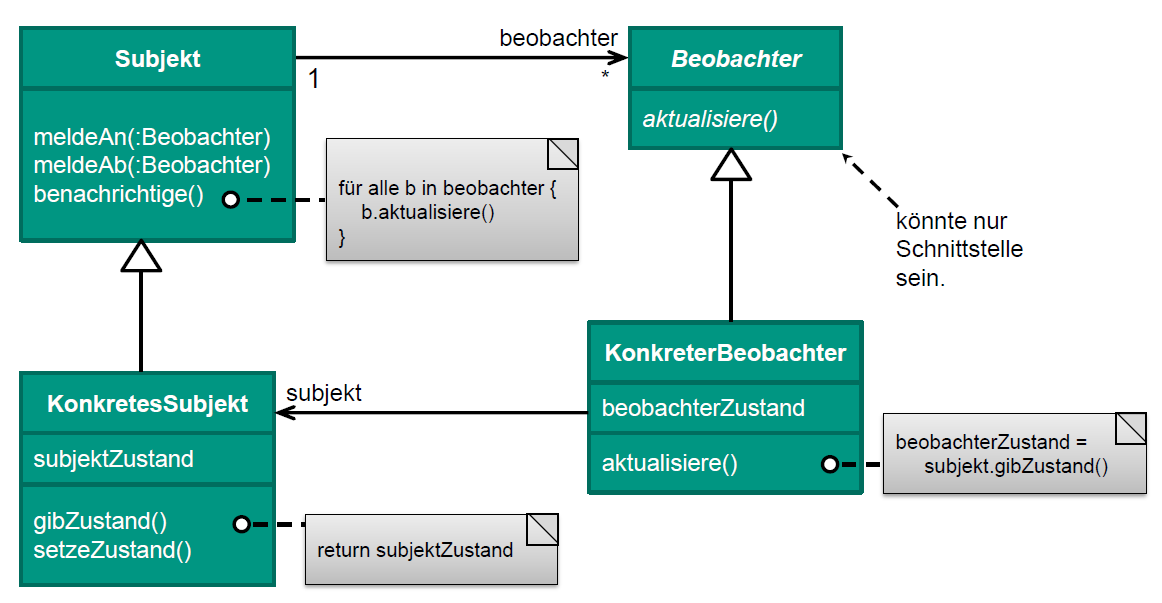
\includegraphics[width=0.9\textwidth]{../resources/images/beobachter.png}
				\end{center}
				\item \textbf{Brücke} (Bridge)
				\begin{itemize}
					\item \textbf{Entkoppelt eine Abstraktion von ihrer Implementierung}, so dass beide \textbf{unabhängig voneinander variiert} werden können
				\end{itemize}
				\begin{center}
					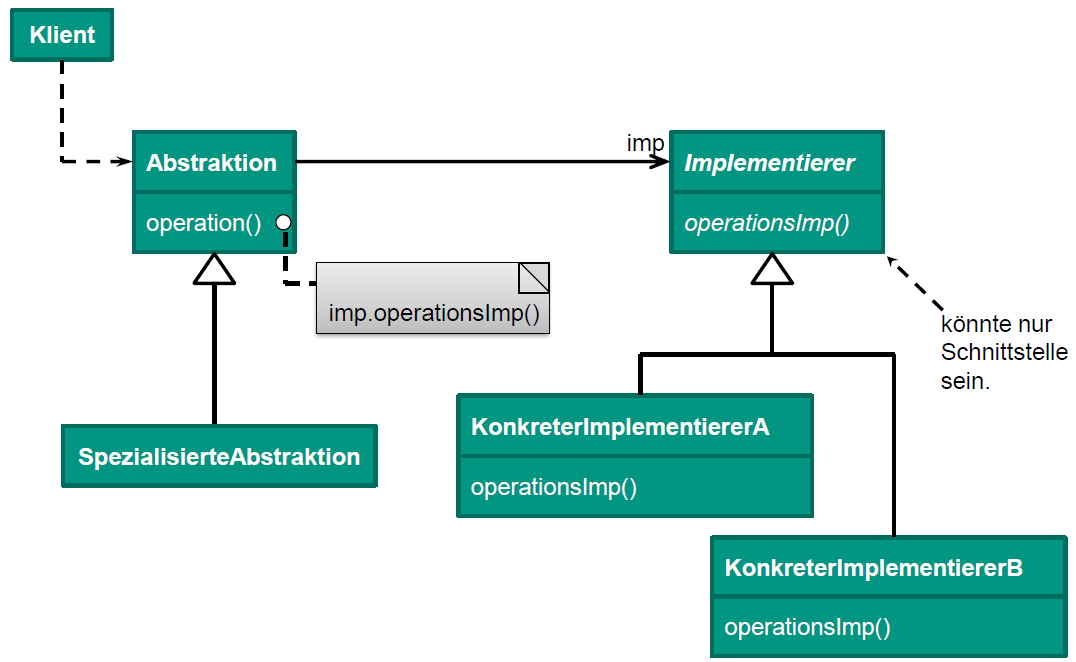
\includegraphics[width=0.8\textwidth]{../resources/images/bruecke.png}
				\end{center}
				\item \textbf{Iterator}
				\begin{itemize}
					\item Ermöglicht \textbf{sequentiellen Zugriff} auf die Elemente eines zusammengesetzten Objektes, \textbf{ohne seine zugrundeliegende Repräsentation offenzulegen}
				\end{itemize}
				\begin{center}
					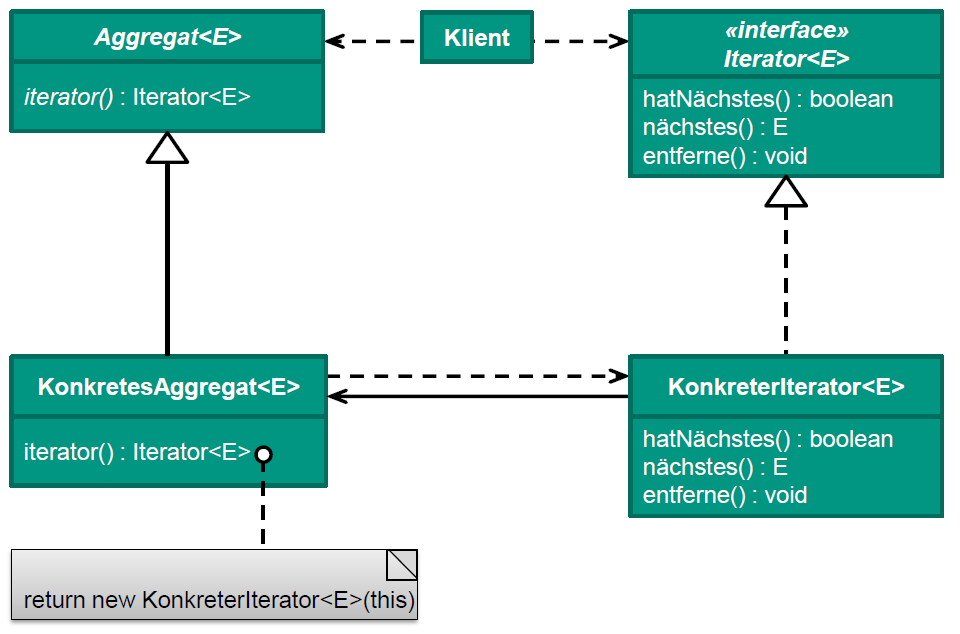
\includegraphics[width=0.7\textwidth]{../resources/images/iterator.png}
				\end{center}
				\item \textbf{Stellvertreter} (Proxy)
				\begin{itemize}
					\item \textbf{Kontrolliert den Zugriff auf ein Objekt}, mit Hilfe eines \textbf{vorgelagerten Stellverteterobjekts}
				\end{itemize}
				\begin{center}
					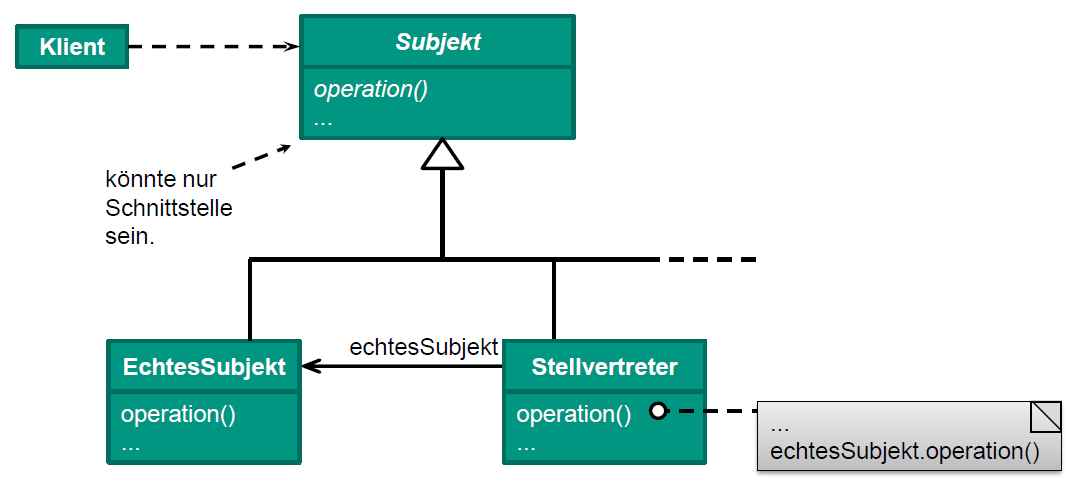
\includegraphics[width=0.9\textwidth]{../resources/images/stellvertreter.png}
				\end{center}
				\item \textbf{Vermittler} (Mediator)
				\begin{itemize}
					\item Definiert ein Objekt, dass das \textbf{Zusammenspiel einer Menge von Objekten} in sich kapselt
					$\Rightarrow$ \textbf{Zentralisieren}!
				\end{itemize}
				\begin{center}
					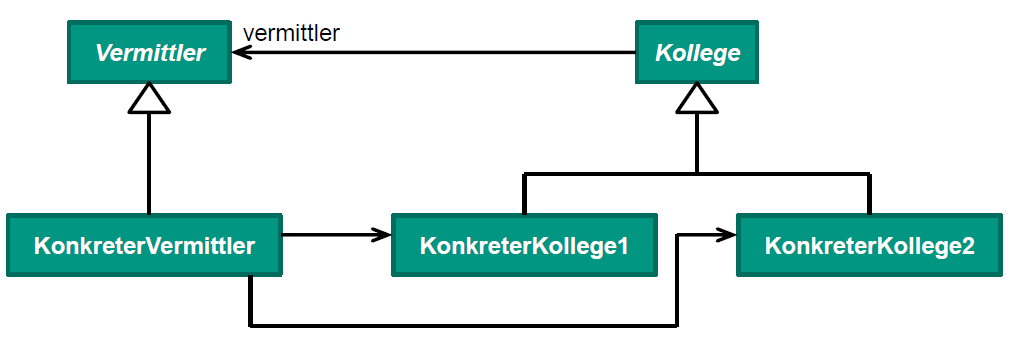
\includegraphics[width=0.9\textwidth]{../resources/images/vermittler.png}
				\end{center}
			\end{itemize}
					
		\newpage
		\subsubsection{Variantenmuster}
				
			\begin{itemize}
				\item \textbf{Abstrakte Fabrik}
				\begin{itemize}
					\item Bietet eine Schnittstelle zum \textbf{Erzeugen von Familien} \underline{verwandter} oder \newline \underline{voneinander abhängigen Objekte}, ohne ihre konkreten Klassen zu benennen
				\end{itemize}
				\begin{center}
					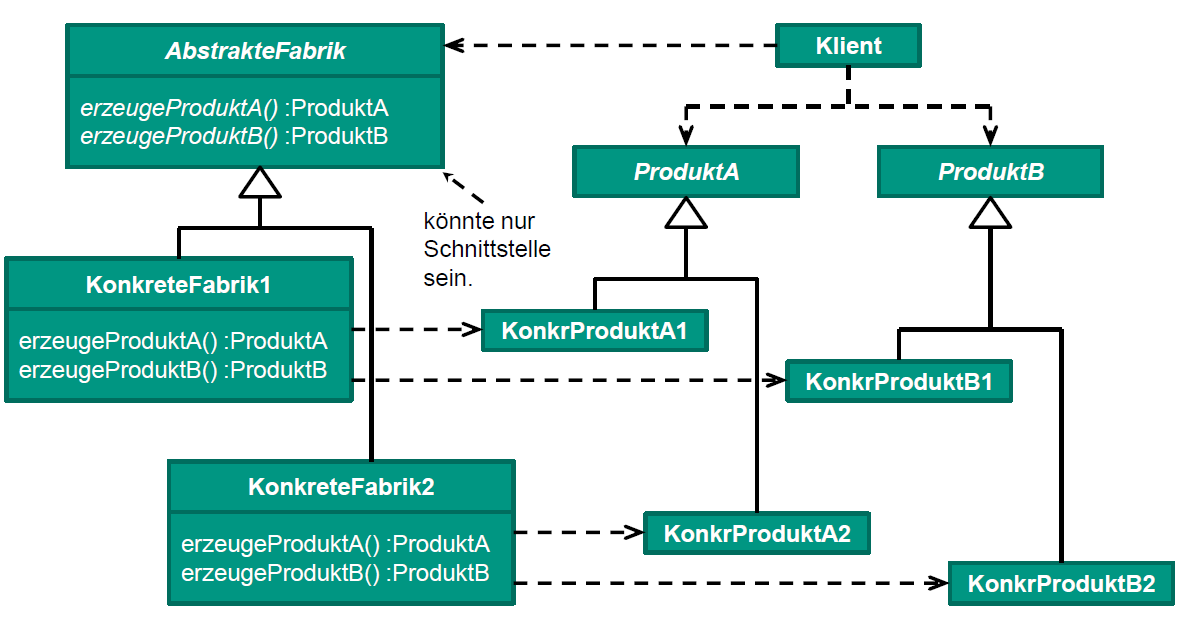
\includegraphics[width=0.8\textwidth]{../resources/images/abstrakteFabrik.png}
				\end{center}
				\item \textbf{Besucher} (Visitor)
				\begin{itemize}
					\item \textbf{Kapselt} eine auf den Elementen einer Objektstruktur \textbf{auszuführenden Operation} als ein Objekt
				\end{itemize}
				\begin{center}
					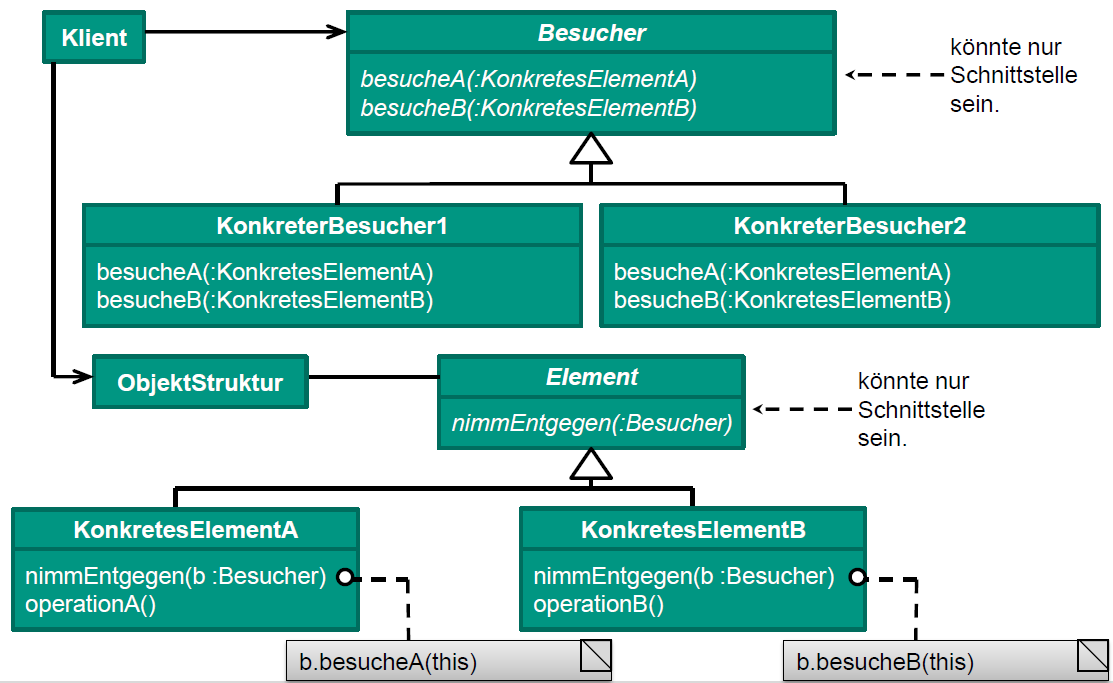
\includegraphics[width=0.8\textwidth]{../resources/images/besucher.png}
				\end{center}
				\item \textbf{Schablonenmethode} (Template Method)
				\begin{itemize}
					\item Definiert \textbf{in einer Methode das Skelett eines Algorithmus} und überlässt einzelne Schritte den Unterklassen
				\end{itemize}
				\begin{center}
					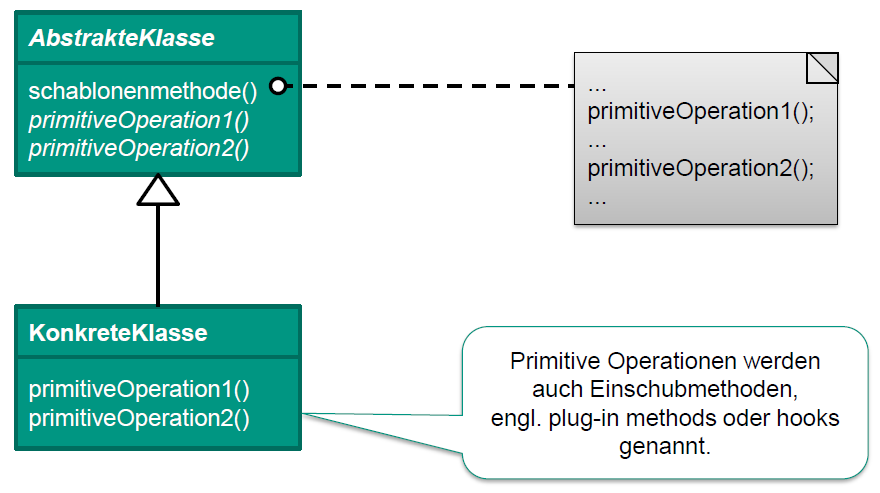
\includegraphics[width=0.9\textwidth]{../resources/images/schablonenmethode.png}
				\end{center}
				\item \textbf{Fabrikmethode} (Factory Method)
				\begin{itemize}
					\item Definiert eine \textbf{Klassenschnittstelle mit Operationen zum Erzeugen} eines Objekts, aber \textbf{lässt Unterklassen entscheiden, von welcher Klasse} das zu erzeugende Objekt ist
				\end{itemize}
				\begin{center}
					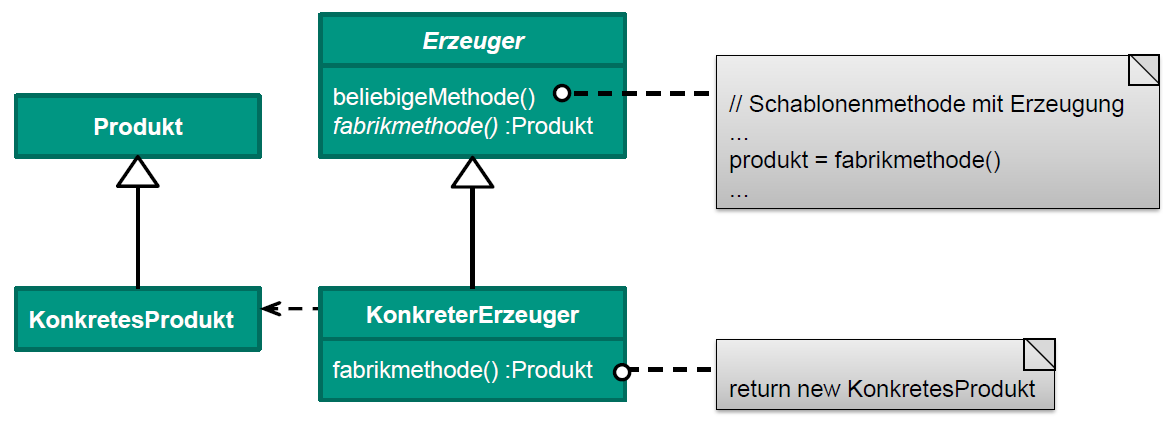
\includegraphics[width=0.9\textwidth]{../resources/images/fabrikmethode.png}
				\end{center}
				\newpage
				\item \textbf{Kompositum}
				\begin{itemize}
					\item Fügt Objekte zu \textbf{Baumstrukturen} zusammen, um \textbf{Bestandshierarchien} zu repräsentieren. Ermöglicht, das \textbf{Klienten, einzelne Objekte und Aggregate einheitlich} behandelt werden
				\end{itemize}
				\begin{center}
					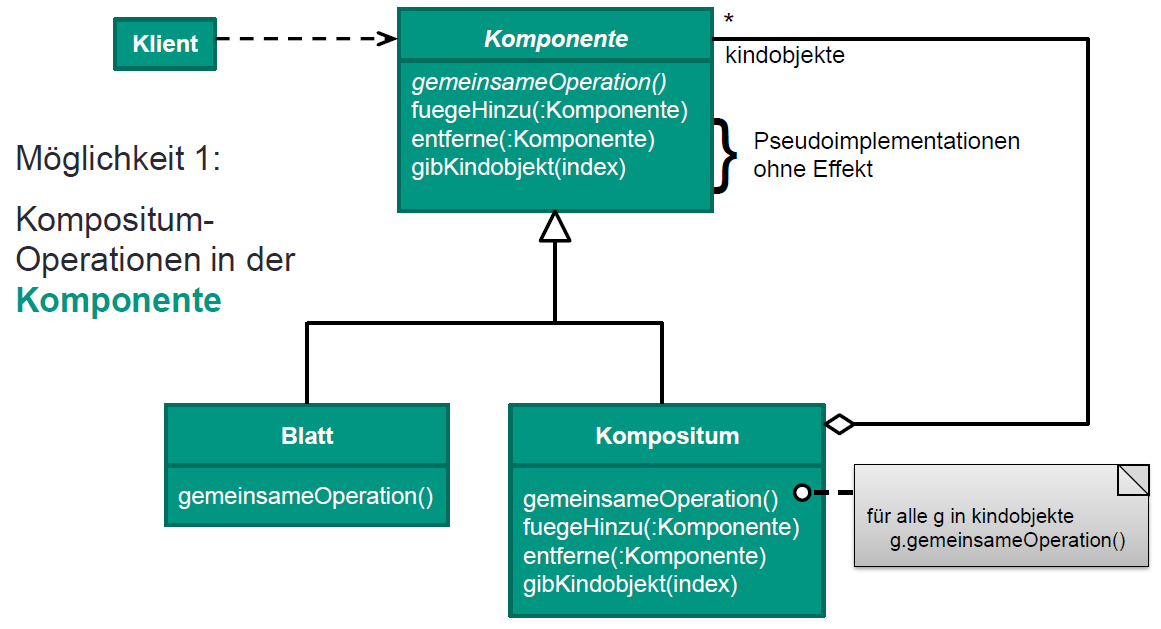
\includegraphics[width=0.9\textwidth]{../resources/images/kompositum.png}
				\end{center}
				\item \textbf{Strategie} (Stichwort: Switch-less programming)
				\begin{itemize}
					\item Definiert eine \textbf{Familie von Algorithmen}, \textbf{kapselt} sie und macht sie \textbf{austauschbar}
				\end{itemize}
				\begin{center}
					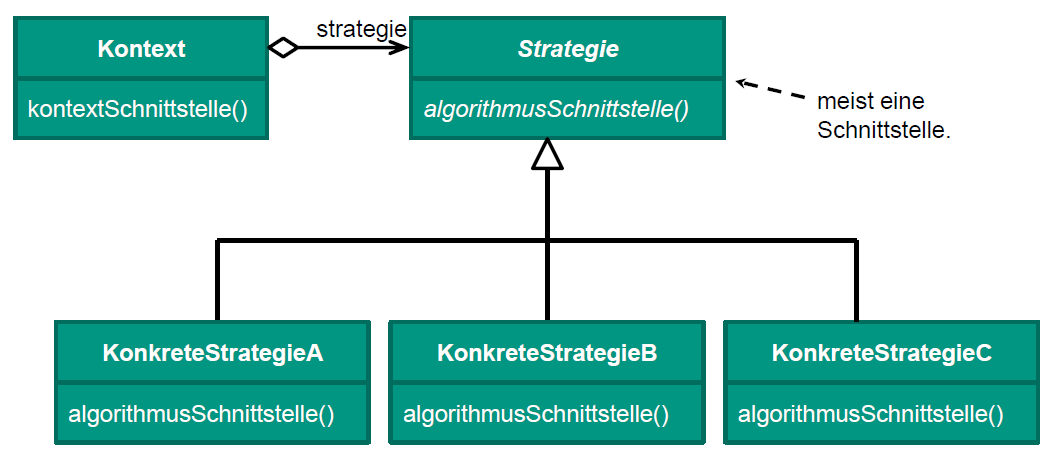
\includegraphics[width=0.9\textwidth]{../resources/images/strategie.png}
				\end{center}
				\newpage
				\item \textbf{Dekorierer}
				\begin{itemize}
					\item Fügt \textbf{dynamisch zur Laufzeit neue Funktionalitäten} zu einem Objekt hinzu
				\end{itemize}
				\begin{center}
					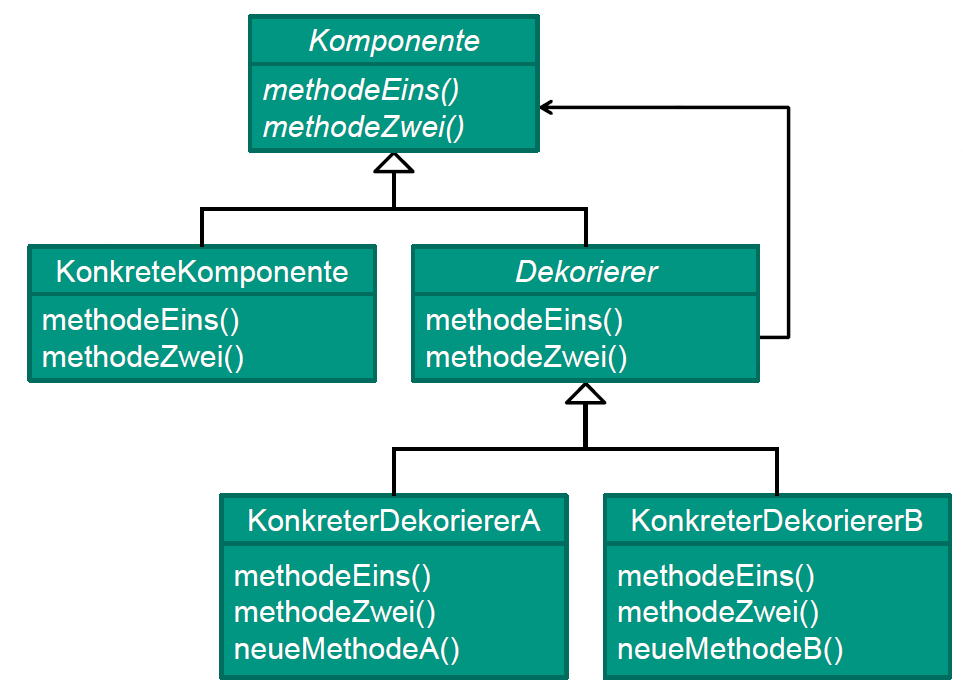
\includegraphics[width=0.6\textwidth]{../resources/images/dekorierer.png}
				\end{center}
			\end{itemize}
					
		\subsubsection{Zustandshandhabungsmuster}
					
			\begin{itemize}
				\item \textbf{Einzelstück} (Singleton)
				\begin{itemize}
					\item Zusicherung, dass eine Klasse \textbf{genau ein Exemplar} besitzt mit \textbf{globalen Zugriffspunkt}
				\end{itemize}
				\begin{center}
					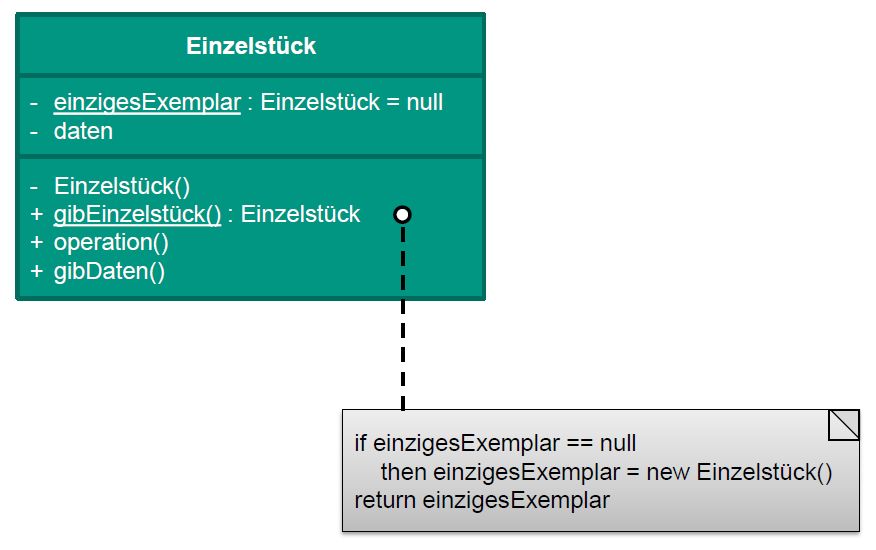
\includegraphics[width=0.7\textwidth]{../resources/images/einzelstueck.png}
				\end{center}
				\newpage
				\item \textbf{Fliegengewicht}
				\begin{itemize}
					\item Nutzt Objekte \textbf{kleinster Granularität gemeinsam}, um große Mengen von ihnen \textbf{effizient zu speichern}
				\end{itemize}
				\begin{center}
					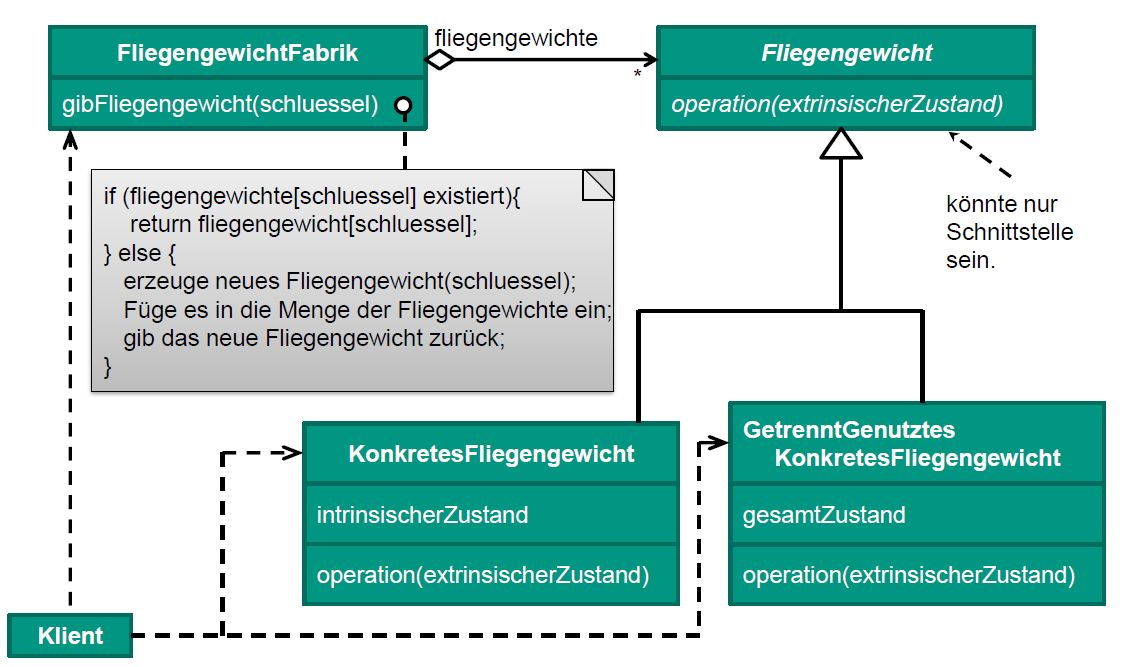
\includegraphics[width=0.8\textwidth]{../resources/images/fliegengewicht.png}
				\end{center}
				\item \textbf{Memento}
				\begin{itemize}
					\item Erfasst und \textbf{externalisiert den internen Zustand eines Objekts}, ohne seine Kapselung zu verletzten, so dass das Objekt \textbf{später in diesen Zustand zurückversetzt} werden kann
				\end{itemize}
				\begin{center}
					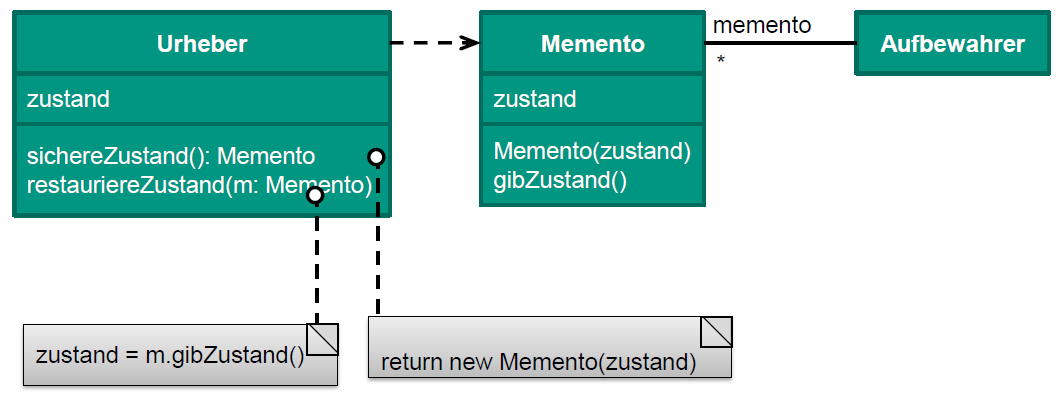
\includegraphics[width=0.9\textwidth]{../resources/images/memento.png}
				\end{center}
				\newpage
				\item \textbf{Prototyp}
				\begin{itemize}
					\item Bestimmt die \textbf{Arten zu erzeugender Objekte} durch die Verwendung eines typischen Exemplars und erzeuge neue Objekte durch \textbf{Kopieren dieses Prototyps}
				\end{itemize}
				\begin{center}
					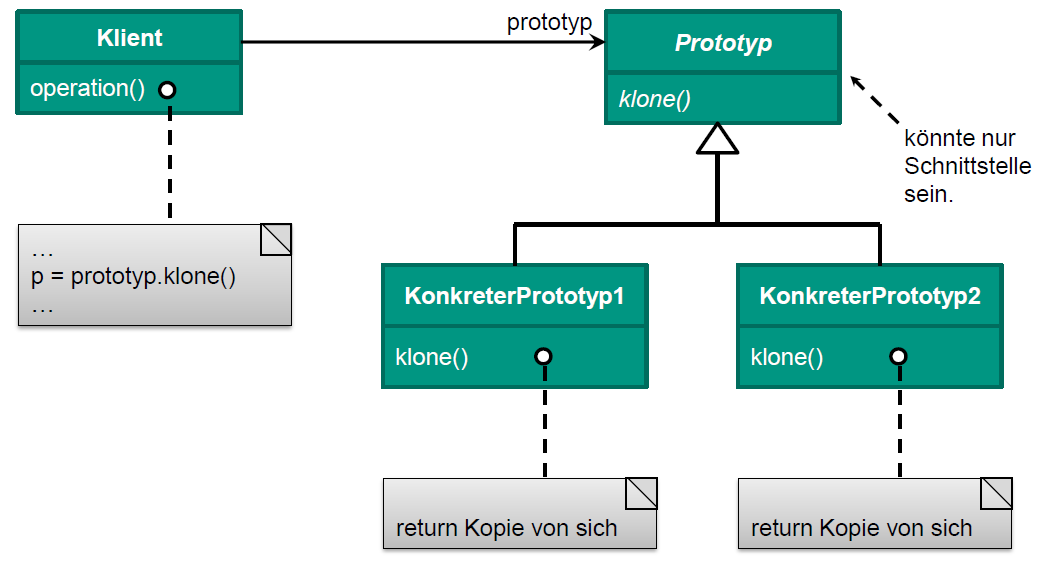
\includegraphics[width=0.9\textwidth]{../resources/images/prototyp.png}
				\end{center}
				\item \textbf{Zustand}
				\begin{itemize}
					\item Ändere das \textbf{Verhalten} des Objekts, wenn sich dessen \textbf{interner Zustand ändert}
				\end{itemize}
				\begin{center}
					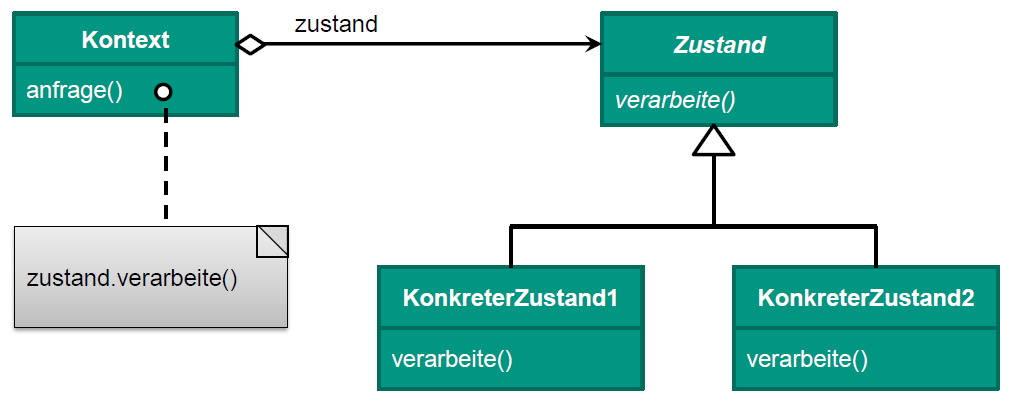
\includegraphics[width=0.9\textwidth]{../resources/images/zustand.png}
				\end{center}
			\end{itemize}
					
		\subsubsection{Steuerungsmuster}
					
			\begin{itemize}
				\item \textbf{Befehl}
				\begin{itemize}
					\item Kapselt einen \textbf{Befehl als Objekt} und ermöglicht es, Klienten mit verschiedenen \textbf{Anfragen zu parametrisieren}, Operationen in eine \textbf{Warteschlange} zu stellen, ein Logbuch zu führen und \textbf{Operationen rückgängig} zu machen
				\end{itemize}
				\begin{center}
					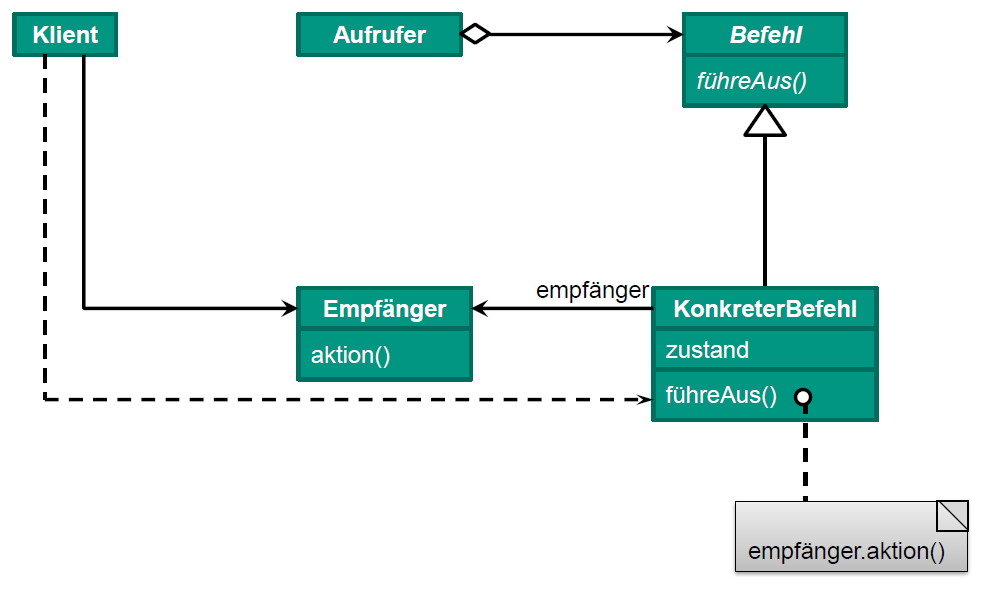
\includegraphics[width=0.7\textwidth]{../resources/images/befehl.png}
				\end{center}
				\item \textbf{Master/Worker}
				\begin{itemize}
					\item Bietet \textbf{fehlertolerante- und parallele Berechnung}. Ein \textbf{Master verteilt die Arbeit an identische Worker} und \textbf{berechnet das Endergebnis} aus den Teilergebnissen, die die Worker zurückliefern
				\end{itemize}
				\begin{center}
					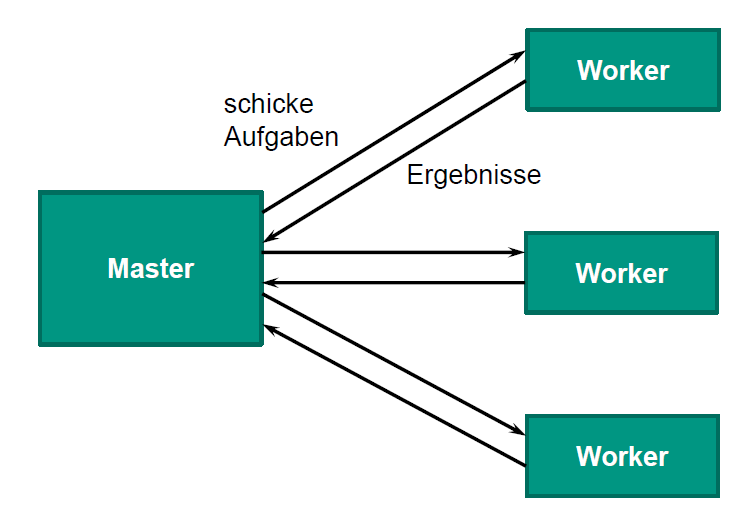
\includegraphics[width=0.6\textwidth]{../resources/images/masterWorker.png}
				\end{center}
			\end{itemize}
			
		\subsubsection{Bequemlichkeitsmuster}
				
			\begin{itemize}
				\item \textbf{Bequemlichkeitsklasse}
				\begin{itemize}
					\item \textbf{Vereinfachung von Methodenaufrufen} durch Bereithaltung der Parameter in \textbf{spezieller Klasse}
				\end{itemize}
				\begin{center}
					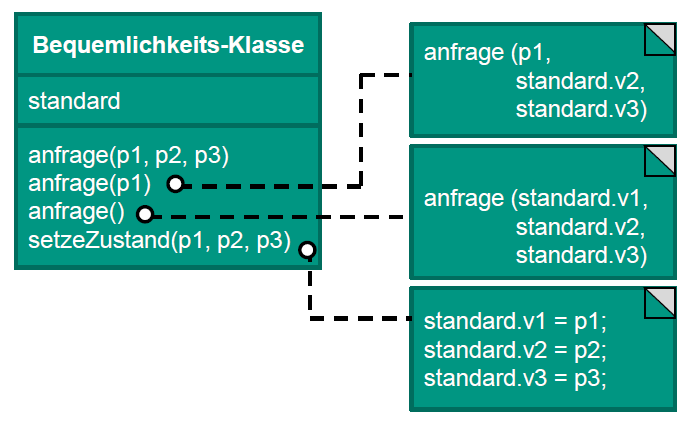
\includegraphics[width=0.8\textwidth]{../resources/images/bequemlichkeitsklasse.png}
				\end{center}
				\item \textbf{Bequemlichkeitsmethode}
				\begin{itemize}
					\item \textbf{Vereinfachung von Methodenaufrufen} durch Bereithaltung \textbf{häufig genutzter Parameterkombinationen} in \textbf{zusätzlichen Methoden}
				\end{itemize}
				\begin{center}
					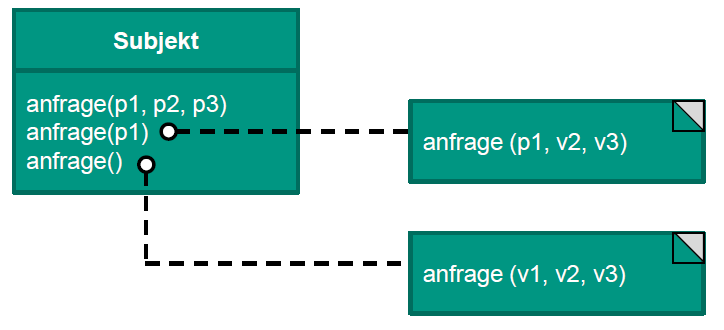
\includegraphics[width=0.8\textwidth]{../resources/images/bequemlichkeitsmethode.png}
				\end{center}
				\newpage
				\item \textbf{Fassade}
				\begin{itemize}
					\item Bietet \textbf{einheitliche Schnittstelle} zu einer \textbf{Menge von Schnittstellen} eines Subsystems
					\begin{itemize}
						\item Fassadenklasse bietet \textbf{abstrakte Schnittstelle}, die die Benutzung des Systems vereinfacht
					\end{itemize}
				\end{itemize}
				\begin{center}
					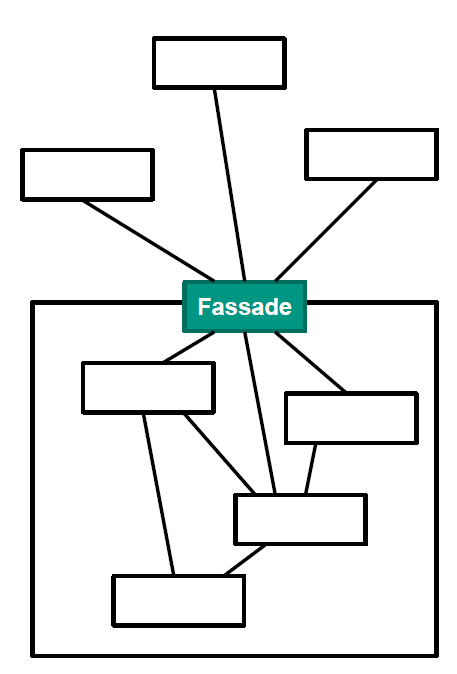
\includegraphics[width=0.3\textwidth]{../resources/images/fassadeSchichtenarchitektur.png}
				\end{center}
				\item \textbf{Null-Objekt}
				\begin{itemize}
					\item Stellt \textbf{Stellvertreter} zur Verfügung, der die gleiche Schnittstelle bietet, aber \textbf{nichts tut}
				\end{itemize}
				\begin{center}
					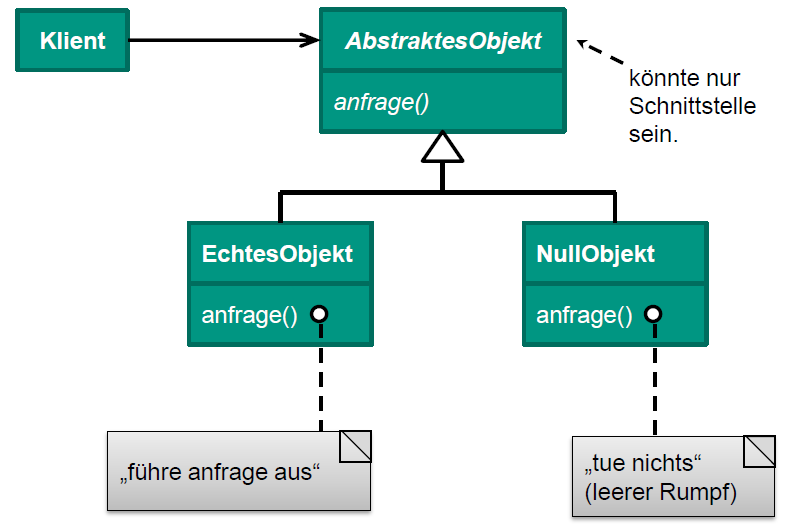
\includegraphics[width=0.6\textwidth]{../resources/images/nullObjekt.png}
				\end{center}
			\end{itemize}